\newpage
\hypertarget{explanation}{}
\section{Transformations explained}
\genHeader

The core idea when modeling behaviour is to regard dynamic aspects of a system (let's call this a model from now on) as bringing about a change of state.
This means a model in state $S$ can evolve to state $S^*$ via a transformation $\Delta: S \stackrel{\Delta}{\rightarrow}S^*$. In this light, dynamic or
behavioural aspects of a model are synonymous with \emph{model transformations}, and the dynamic semantics of a language equates simply to a suitable set of
model transformations. This approach is once again quite similar to the object oriented (OO) paradigm, where objects have a state, and can \emph{do} things via
methods that manipulate their state.

So how do we \emph{model} model transformations?  There are quite a few possibilities. We could employ a suitably concise imperative programming language in
which we simply say how the system morphs in a step-by-step manner. There actually exist quite a few very successful languages and tools in this direction. But
isn't this almost like just programming directly in Java? There's got to be a better way! 

From the relatively mature field of graph grammars and graph transformations, we take a \emph{declarative} and \emph{rule-based} approach. Declarative in this
context means that we do not want to specify exactly how, and in what order, changes to the model must be carried out to achieve a transformation. We just want
to say under what conditions the transformation can be executed (precondition), and the state of the model after executing the transformation (postcondition).
The actual task of going from precondition to postcondition should be taken over by a transformation engine, where all related details are basically regarded as
a black box.

So, inspired by string grammars and this new, refined idea of a model transformation (which is of the form $(pre, post)$), let's call this black box
transformation a \emph{rule}. It follows that the precondition is the left-hand side of the rule, $L$, and the postcondition is the right-hand side, $R$.

A rule, $r: (L,R)$, can be \emph{applied} to a model (a typed graph) $G$ by:
\begin{enumerate}
  \item \emph{Finding} an occurrence of the precondition $L$ in $G$ via a \emph{match}, $m$
  
  \item \emph{Cutting} out or $Destroying$ $(L\setminus R)$, i.e., the elements that are present in the precondition but not in the postcondition are deleted
  from $G$ to form  $(G\setminus Destroy)$
  
  \item \emph{Pasting} or $Creating$ $(R\setminus L)$, i.e., new elements that are present in the postcondition but not in the precondition and are to be created
  in the hole left in $(G\setminus Destroy)$ to form a new graph, $H = (G\setminus Destroy) \cup Create$ (\Cref{fig:rule_application}). 
  
  \end{enumerate}

\vspace{0.5cm}

\begin{figure}[htp]
\begin{center}
  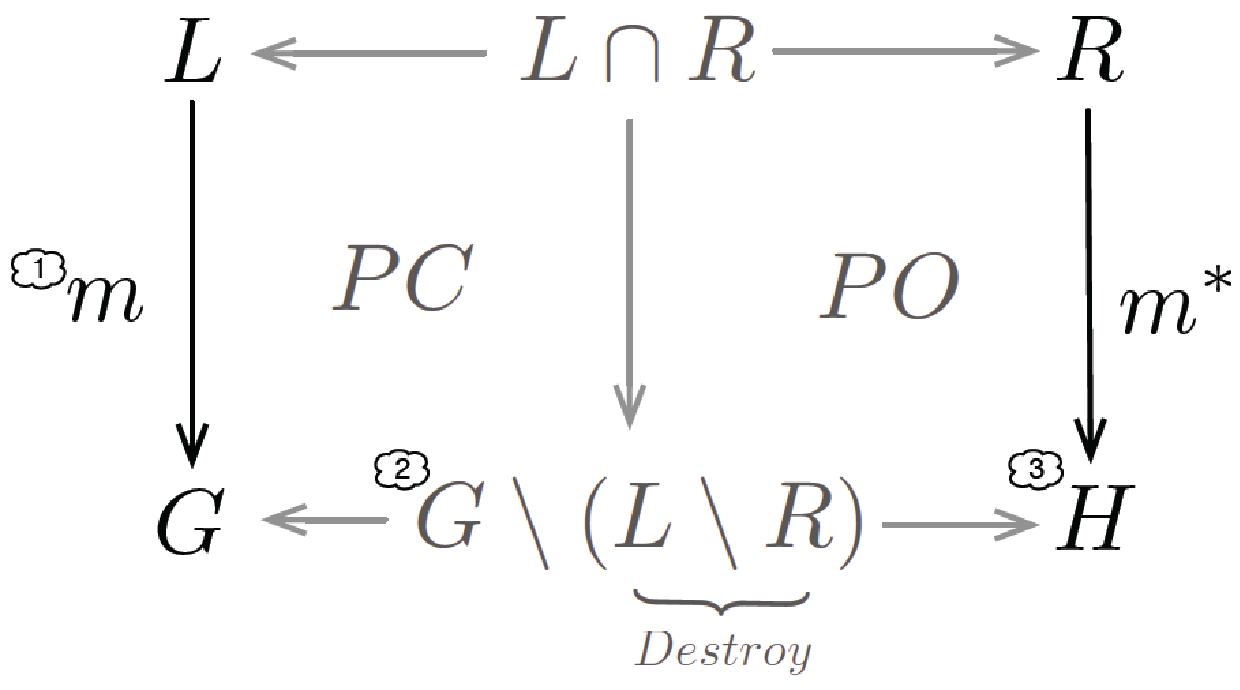
\includegraphics[width=0.8\textwidth]{rule_application}
  \caption[]{Applying a rule $r: (L,R)$ to $G$ to yield $H$} 
  \label{fig:rule_application}
\end{center}
\end{figure}

\vspace{0.5cm}

Let's review this application. 

(1) is determined by a process called \emph{graph pattern matching}\define{Pattern Matching} i.e., finding an occurrence or
\emph{match} of the precondition or \emph{pattern} in the model $G$.

(2) is determined by building a \emph{push-out complement} $PC = (G\setminus Destroy)$, such that $L\cup PC = G$.

(3) is determined by building a \emph{push-out} $PO = H$, so that $(G\setminus Destroy) \cup R = H$.

A push-out (complement) is a generalised union (subtraction) defined on typed graphs. Since we are dealing with graphs, it is not such a trivial task to define
(1) -- (3) in precise terms, with conditions for when a rule can or cannot be applied. A substantial amount of theory already exists to satisfy this goal.

Since this black box formalisation involves two push-outs - one when cutting $Destroy := (L\setminus R)$ from $G$ to yield $(G\setminus Destroy)$ (deletion),
and one when inserting $Create := (R\setminus L)$ in $(G\setminus Destroy)$ to yield $H$ (creation) - this construction is referred to as a \emph{double
push-out}. We won't go into further details in this handbook, but the interested reader can refer to \cite{EEPT06} for the exciting details.

Now that we know what rules are, let's take a look at a simple example for our learning box. What would a rule application look like for moving a card from
one partition to the next? \Cref{fig:rule_example} depicts this $moveCard$ rule.
  
\begin{figure}[htp]
\begin{center}
  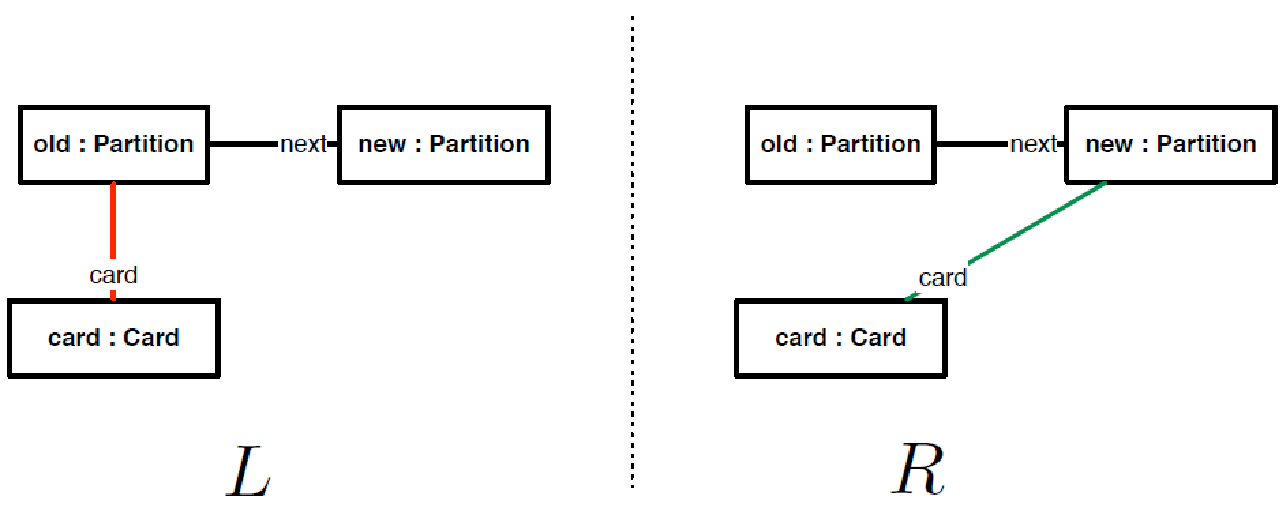
\includegraphics[width=1\textwidth]{rule_example}
  \caption[]{$moveCard$ as a graph transformation rule}	
  \label{fig:rule_example}
\end{center}
\end{figure}


As already indicated by the colours used for $moveCard$, we employ a compact representation of rules formed by merging $(L,R)$ into a single \emph{story
pattern}\define{Story Pattern} composed of  $Destroy := (L\setminus R)$ in red, $Retain :=  L\cap R$ in black, and $Create := (R\setminus L)$ in green
(\Cref{fig:rule_compact}).

\begin{figure}[htp]
\begin{center}
  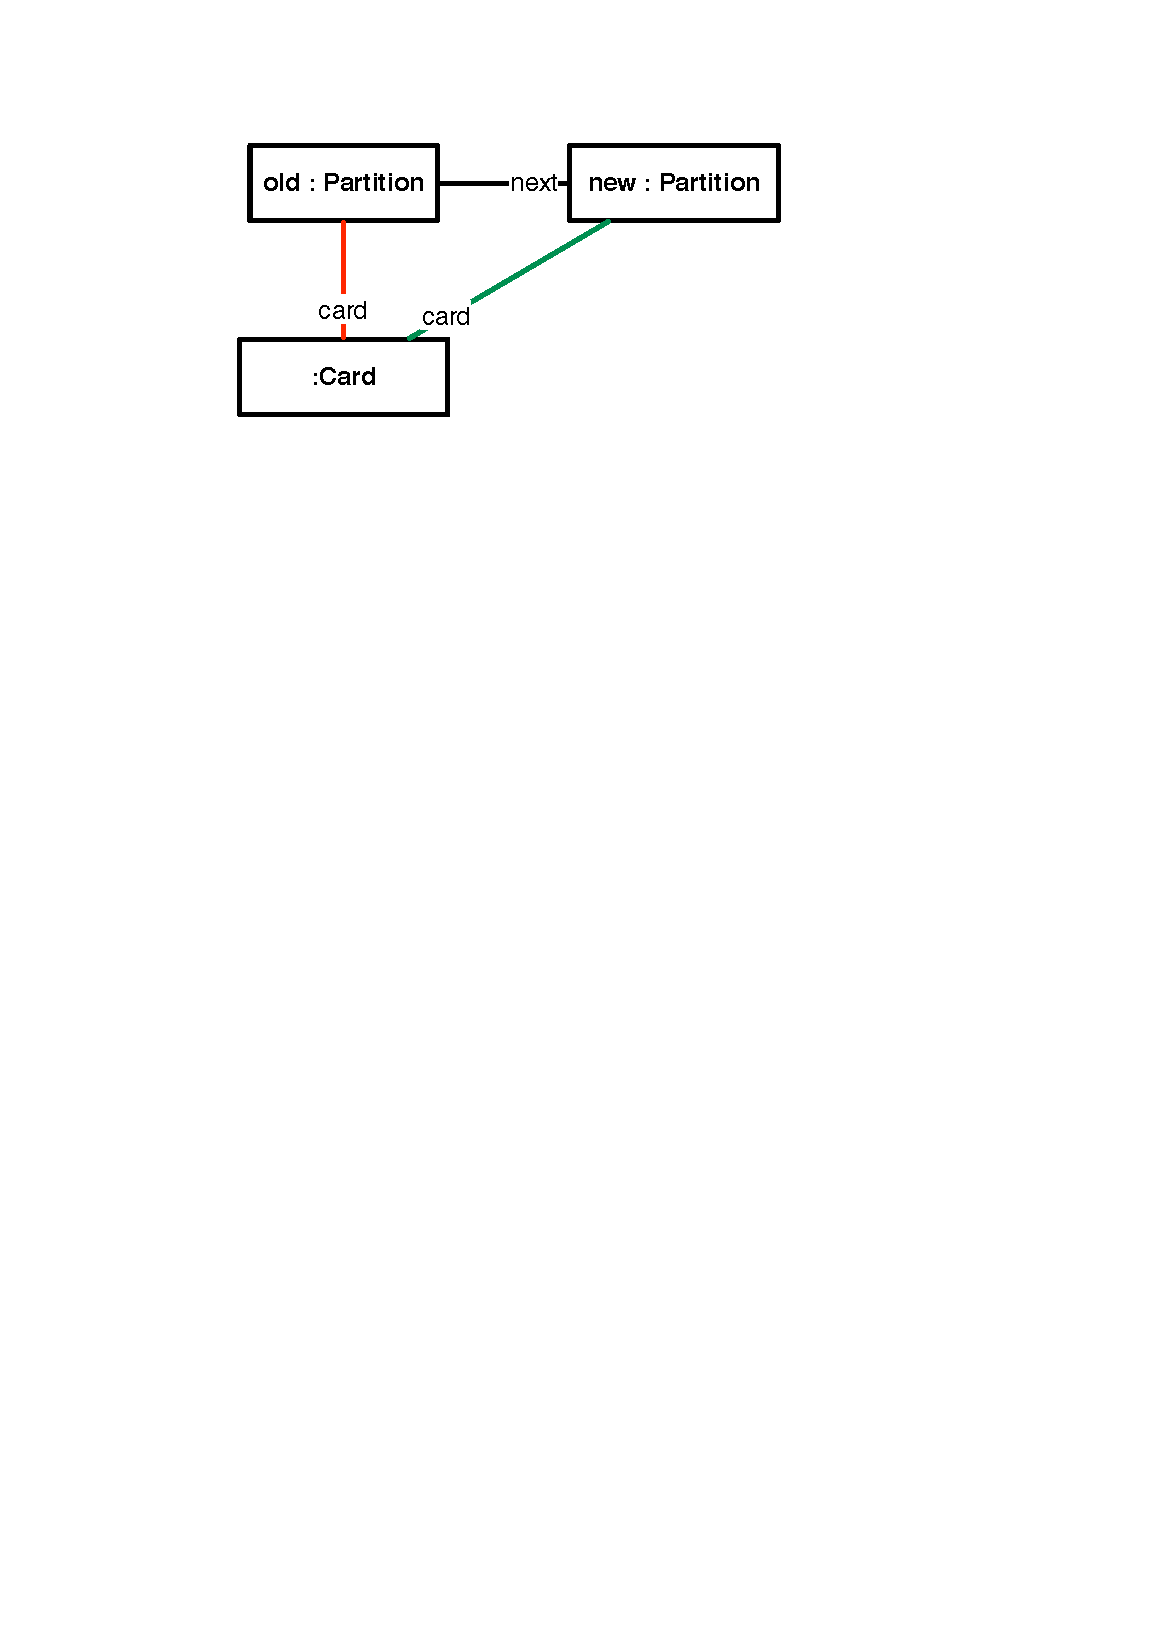
\includegraphics[width=0.45\textwidth]{rule_compact}
  \caption[]{Compact representation of $moveCard$ as a single \emph{story pattern}}
  \label{fig:rule_compact}
\end{center}
\end{figure}

As we shall see in a moment, this  representation is quite intuitive, as one can just forget the details of rule application and think in terms of what is to be
deleted, retained, and created. We can therefore apply $moveCard$ to a learning box in terms of steps (1) -- (3), as depicted in \Cref{fig:rule_app_example}.

Despite being able to merge rules together to form one story pattern, the individual rules still have to be applied in a suitable sequence to realise complex
model transformations consisting of many steps! This can be specified with simplified activity diagrams, where every \emph{activity node}\define{Activity Node}
or \emph{story node} contains a single \emph{story pattern}, and are combined with the usual imperative constructs to form a control flow structure. The entire
transformation can therefore be viewed as two separate layers: an imperative layer to define the top-level control flow via activities (i.e., if/else
statements, loops, etc.), and a pattern layer where each story pattern specifies (via a graph transformation rule) how the model is to be manipulated.

\pagebreak

\vspace*{2cm}

\begin{figure}[htp] 
\begin{center}
  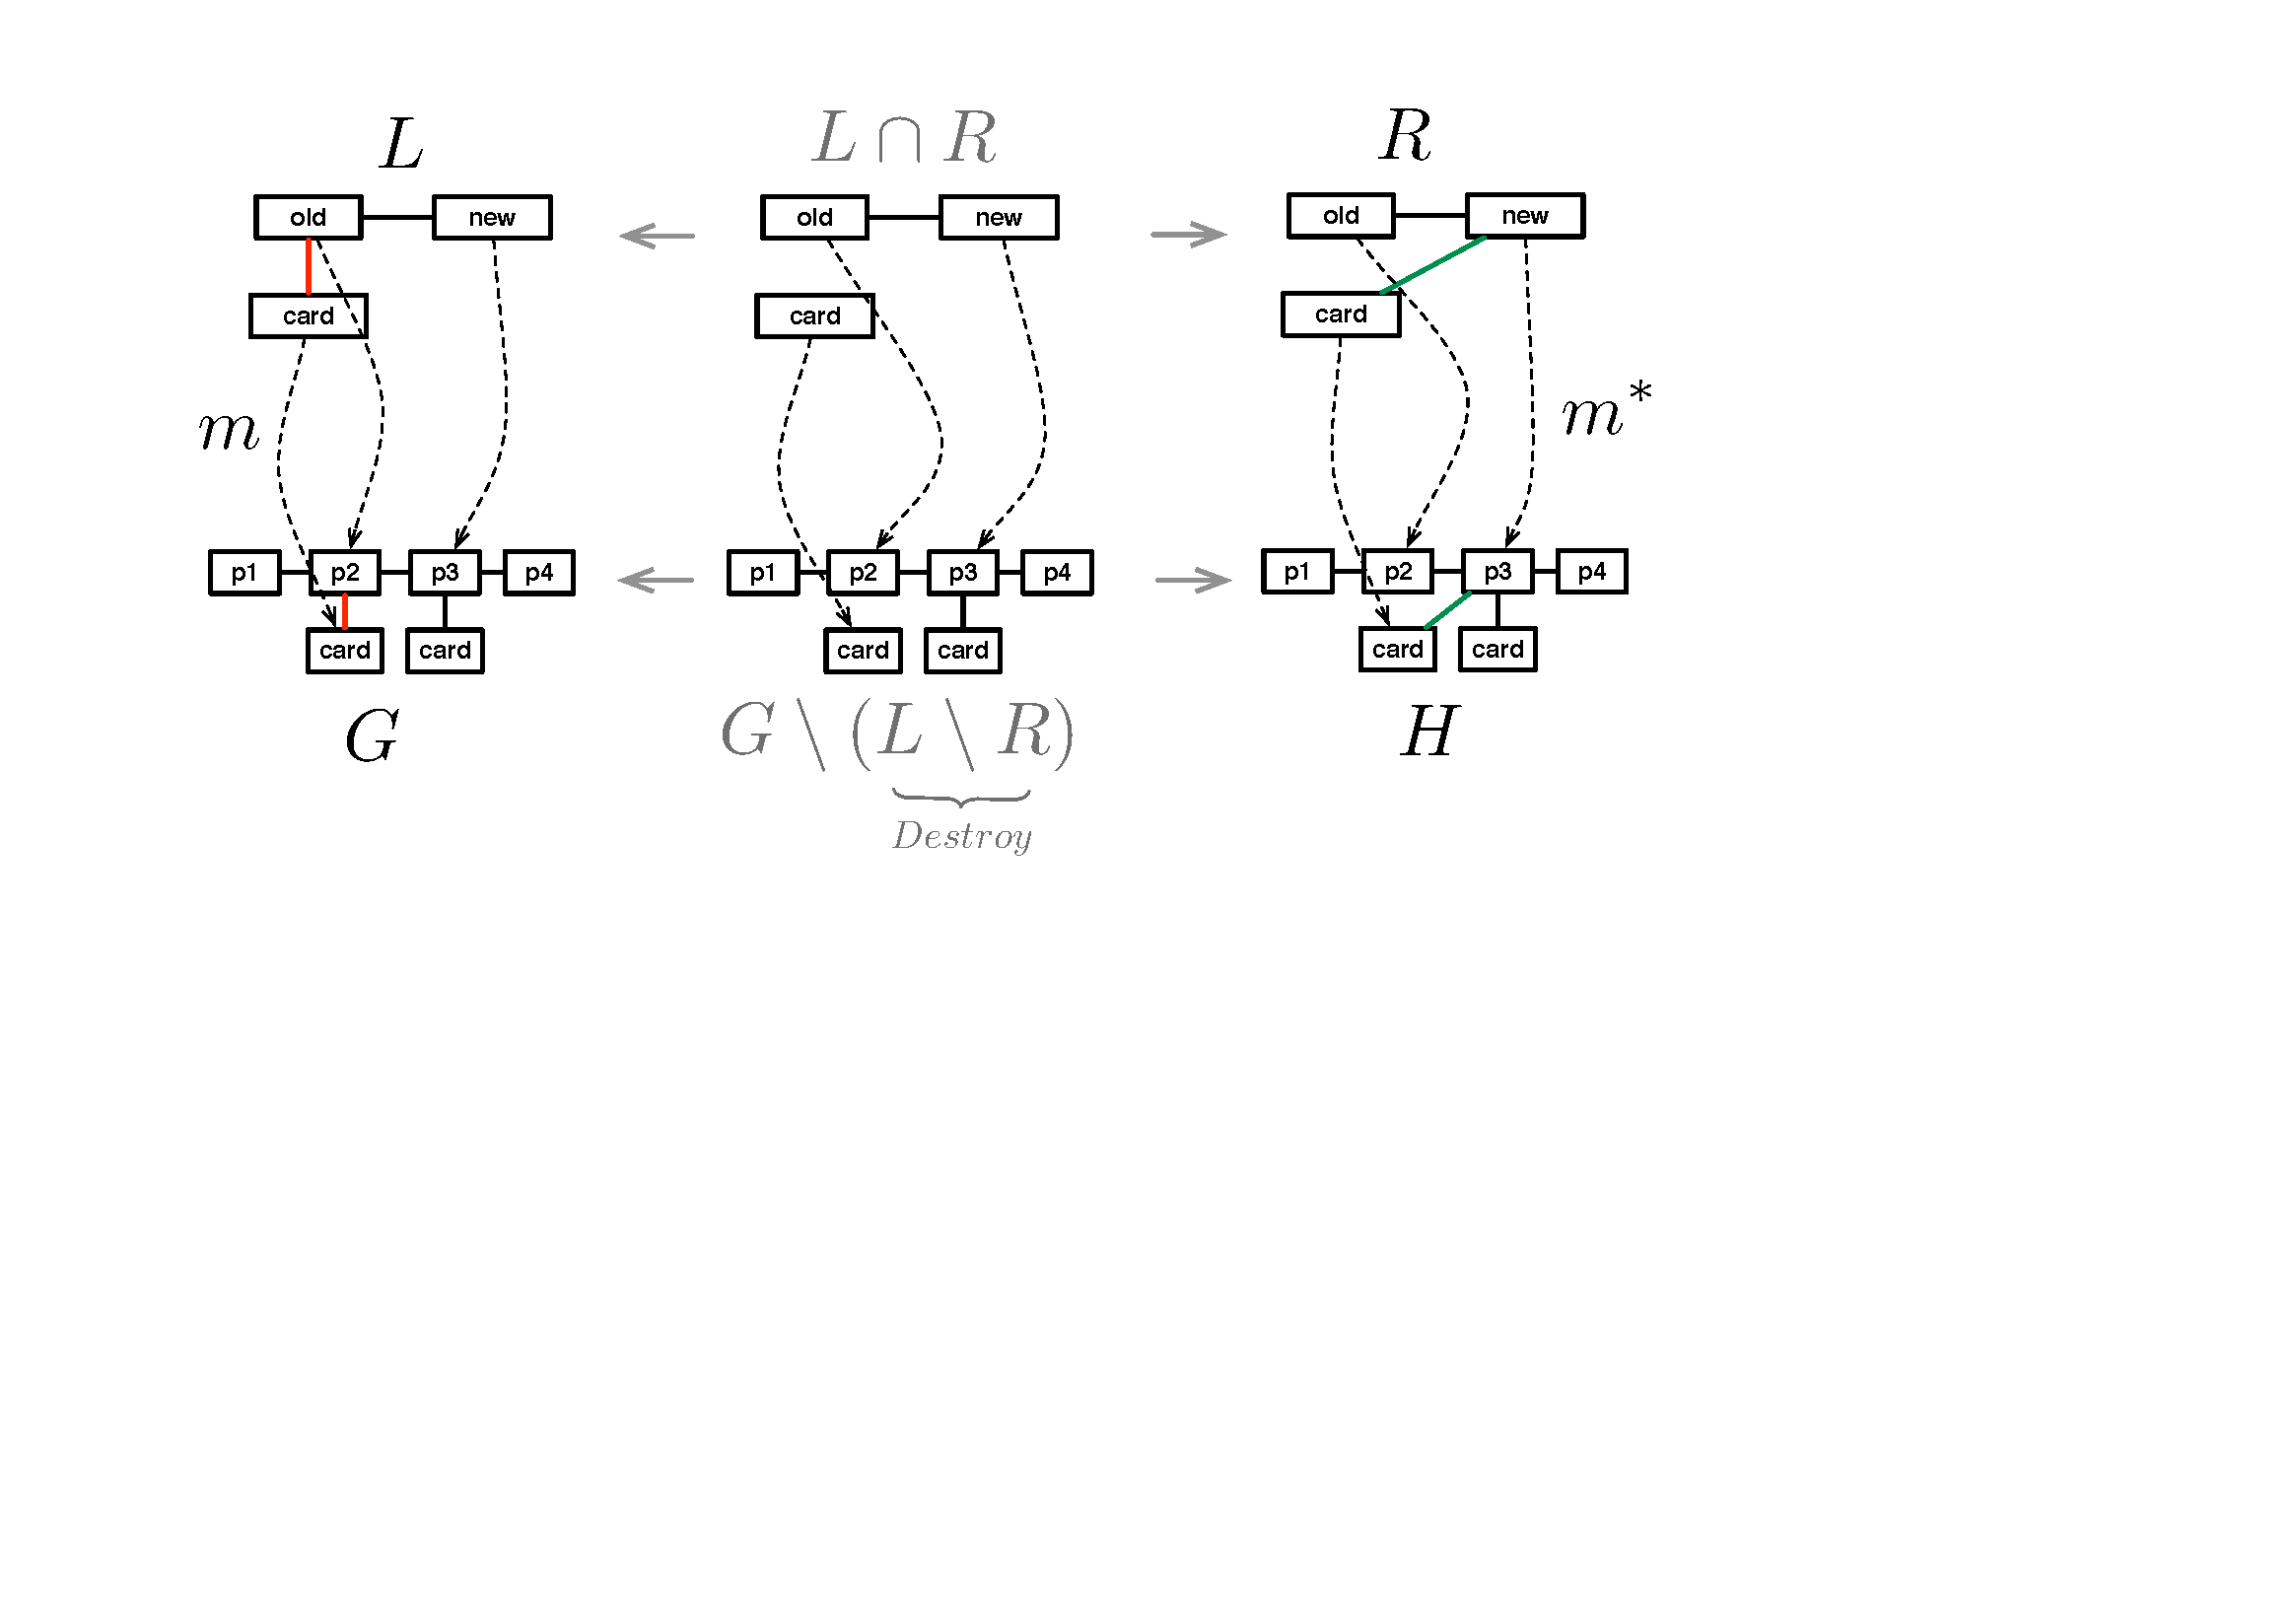
\includegraphics[width=1\textwidth]{rule_app_example}
  \caption[]{Applying $moveCard$ to a learning box}
  \label{fig:rule_app_example}
\end{center}
\end{figure}

\vspace*{1cm}

Enough theory! Grab your mouse and let's get cracking with SDMs\ldots
